\chapter{Oszthatlan közösen készített programok}\label{chap:oszthatlan_kozos_dolgok}

\section{A nyelvi séma átírása}

\noindent

A JSAN a JavaScriptSchemára épül. Ha valamit meg akarunk változtatni gyökerestül a JSANba, akkor a schémát is változtatni kell.
Azt elérni, hogy javascript mellett még typescriptes kódokat is elemezzen a JSAN, ahhoz gyökerestül meg kellett változtatni a JavaScript Analyzert.
Az előző JavaScriptSchema (ami csak javascriptet elemzett) az a javascript hivatalos oldala alapján készült. Ami ábrák fentebb megtalálhatóak, azok már az átírt schémából vannak.
Több opció is volt, hogy most vagy legyen átírva a schéma, vagy legyen egy külön typescriptre is írva.
Végül rájöttünk, hogy ha van egy typescriptes schémánk, az képes javascriptet ugyanúgy elemezni ha megfelelően van lefejlesztve.
Így egy schémát fejlesztettünk le. Az előző schéma átláthatatlan volt, ezért úgy döntöttünk, hogy majdnem a nulláról újraírjuk.
Egyedül a base packaget emeltük át a régiből, BaseNode-al és BaseTokennel kibővítve (\Aref{fig:base_vpp} ábrán látható).
Emellett el kellett dönteni, hogy milyen struktúrát kövessünk, ami jól átlatható és később könnyebben bővíthető.
Végül a typescript-eslint official github alapján haladtunk. Annyi változtatással, hogy ami nekik a base mappában volt, mi arra létrehoztunk egy külön structure packaget.
Mindenhez készítettünk dokumentációt, jól érthetően leírtuk, hogy mit miért kellett csinálni.
Mivel minden is egymásra épül a typescriptes schémában, ezért nem tudtuk tesztelni minden egyes package után, hogy működik-e vagy sem.
Mint például, látható \aref{lst:asg_file_export_all_declaration} kódrészleten, hogy az ExportAllDeclaration mennyi mindenből származik le vagy mennyire sok attribútuma van.
Az ExportAllDeclaration egyik attribútuma, az assertions típusa az ImportAttribute. Ahhoz, hogy jól észrevegye az ExportAllDeclarationt az Analyzer, ahhoz jól le kellett fejleszteni az ImportAttributet.

\begin{lstlisting}[caption={ImportAttribute},label={lst:asg_file_import_attribute}, language={JavaScript}]
export interface ImportAttribute extends BaseNode {
      type: AST_NODE_TYPES.ImportAttribute;
      key: Identifier | Literal;
      value: Literal;
}
\end{lstlisting}
Ahhoz, hogy az ImportAttributet letudjuk fejleszteni a schémában, ahhoz le kell fejleszteni az Identifiert, és a Literalt.
Kicsit összetett, hogy mi minden épül egymásra. Ebből adódik a következő alfejezet mondandója is.

\section{Nehézségek, problémák}

\noindent

A schéma átírása során több nehézségbe is ütköztünk.
A legelső nehézség az a Visual Paradigm program korrekt használata volt.
Egy kisebb időbe tellett rájönni arra, hogy egy adott classnak hogyan kell megváltoztatni a háttérszínét, packagek közötti mozgást, hogyan kell egy adott classra hivatkozni ami másik packageben volt.
Ezután ami szerintem a legnagyobb nehézség volt, az az, hogy nem volt dokumentáció az előző schémához.
Mindent nekünk kellett kitalálni, hogy mit miért csináltak az előző fejlesztők. Akik ezt a schémát fejlesztették le, ők már nem foglalkoztak ezzel, és más nem nagyon mélyedt bele ebbe az egészbe azóta.
A következő nagyobb nehézség, az az volt, hogy összehozzunk egy olyan schémát ami működőképes, és az analyzer ezt tudja is használni.
Előző alfejezetben említettem, hogy egy adott classt (mint például ExportAllDeclaration) lefejlesszünk, ahhoz sok minden mást is le kell fejleszteni, amihez meg még több minden kellett.
Ebből adódóan tesztelni nagyon nem tudtunk, mivel az egésznek működnie kellett ahhoz, hogy az analyzer egyáltalán lefusson.
Mivel mi majdnem nulláról írtuk újra, ez volt a hátrány.
Amikor elérkeztünk ahhoz az állapothoz, hogy mindenre rámondjuk azt, hogy működik, akkor jött egy nagyobb probléma.
Valahol Segmentation Fault-ot kapott a program, és nem nagyon tudtuk ezt debugolni.
Több sejtésünk is volt, hogy mi lehet a baj. Emiatt az egész schémát át kellett nézni alaposan, hogy hol vétettünk hibákat.
Sok helyen voltak pontatlanságok, rossz osztályból származtattunk le, rossz típus volt megadva attribútumnak. Ezeket mind kijavítottuk, de most már más hibát kaptunk.
A JavaScript Analyzerben kiderítettük, hogy pontosan hol szállt el a program.
A Literal volt a hiba, mivel ezt nem a github alapján írtuk meg, hanem egyedi ötlettel. Előző schémában is máshogy volt megoldva.
\begin{figure}[!htbp]
      \caption{A DataStructures packageben a Kind package felépítése}\label{fig:literal}
      \centering
      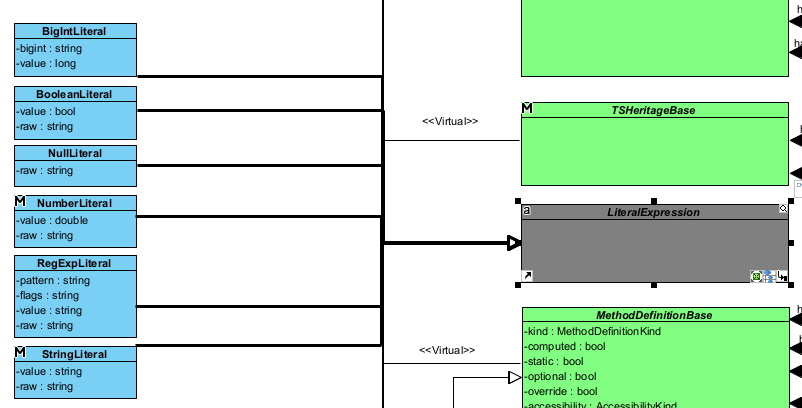
\includegraphics[width=0.8\textwidth]{literal.png}
\end{figure}

\Aref{fig:literal} ábrán látható, hogy a LiteralExpressionből (Ami a Literal) több literal is öröklődik.
\begin{lstlisting}[caption={Literal},label={lst:asg_file_literal}, language={JavaScript}]
export interface LiteralBase extends BaseNode {
  type: AST_NODE_TYPES.Literal;
  raw: string;
  value: RegExp | bigint | boolean | number | string | null;
}
\end{lstlisting}
Próbáltuk úgy megoldani, hogy 4 vagyolással 4 különböző literál tartalmazza, de az analyzerben máshogy kezeltük le a literalt, mint nodeot.
Ezért a tartalmazás helyett inkább örököltettünk a literalból, így megoldva ezt a problémát.
Még az is probléma volt, hogy volt egy LiteralBaseünk, amiből származott ez az 5 literal. A LiteralBase származott a LiteralExpressionből, de valamiért Segmentation fault lett a vége ha így próbáltuk megoldani.
Ezért a LiteralBase-t kivettük, és LiteralExpressionből származik minden literal.
Végül még az volt a nehézség, hogy kódrészletet keressünk az analyzernek, amin le tudjuk tesztelni, hogy az analyzer jó outputot ad-e.

\noindent

Mivel nem nagyon volt typescriptes háttértudásunk, először a typescriptet kellett átnézni, hogy mit hogyan tudunk megvalósítani.
Emellett még a javascriptes outputokat is át kellett nézni, mivel a mi célunk a fejlesztés volt. A jelenlegi javascriptes projektekre ugyanolyan eredményt adott, sőt néhány helyen jobbat is, mert az előző schémában is voltak pontatlanságok.
A typescriptes projektek nagy részét tudja elemezni az analyzer, de közel sem tökéletes, mivel egyfolytában kellene fejleszteni a schémát, mivel a typescript nem annyira régi.


